\newpage
%%%%%%%%%%%%%%%%%%%%%%%%%%%%%%%%%%%%%%%%%%%%%%%%%%%%%%%%%%%%%%%%%%%%%%%%%%%%%%%%
%%%%%%%%%%%%%%%%%%%%%%%%%%%%%%%%%%%%%%%%%%%%%%%%%%%%%%%%%%%%%%%%%%%%%%%%%%%%%%%%
\section{Percepção de frases musicais}
\label{sec:perceberfrases}
\index{Musicalidade!Frase musical}

Como foi visto na Seção \ref{sec:Frase}, 
as \hyperref[sec:Frase]{\textbf{frases musicais}} podem ser classificadas seguindo seu tipo de inicio e final. 
A composição estruturada que envolve os critérios que são usados para agrupar frases musicais em estruturas maiores 
é estudada nas seções \ref{sec:fraseio}, \ref{sec:estruturadamusica} e \ref{sec:compondoestruturadamente}. 
Um par de exemplos simples destas estruturas formadas por frases 
foram vistos quando estudamos os \hyperref[sec:Periodo]{\textbf{períodos}} e 
as \hyperref[sec:sentence]{\textbf{sentenças}} nas Seções \ref{sec:Periodo} e \ref{sec:sentence}, 
respetivamente.

Nesta seção presentaremos critérios para poder dividir uma música ou uma seção dela 
nas suas frases musicais. 


\begin{tcbattention}
Uma coisa importante a ter em conta quando analisamos as frases numa música 
é que estas tendem a ser percebidas de forma irregular na introdução da música;
porque nessa seção da peça os compositores tem muita liberdade criativa
e costumam introduzir irregularidades no comprimento da frase em relação ao corpo da peça. 
Por isso é recomendável iniciar nosso analises das frases no corpo da música. 
\end{tcbattention}

\subsection{Separando frases analiticamente}

Para poder identificar as frases musicais,
nesta seção serão presentadas algumas dicas extraídas da teoria musical,
pelo que seu uso requer um mínimo de conhecimento teórico nesta área. 



\PRLsep{Frases de comprimento regular}

Na música popular, podemos achar peças com frases musicais com um comprimento regular,
ou seja que  tem a mesma quantidade de compassos em toda a música;
nesse caso, uma forma de identificar e separar as frases musicais  
é detetando uma frase na peça musical,
contar o número de compassos que esta contem  
e usar esta medida para detetar e predizer as demais frases.


\begin{itemize}
\item Os comprimento de frase de 4 e 8 compassos 
são os mais comuns de serem vistos
\cite[pp. 624]{latham2008diccionario} \cite[pp. 335]{medteoria} \cite[pp. 34]{bennett1993elementos} %4
\cite[pp. 335]{medteoria} \cite[pp. 34]{bennett1993elementos}. %8
\item São incomuns frases de 3, 5, ou 7 compassos \cite[pp. 34]{bennett1993elementos}.
\end{itemize}
Assim, quando iniciemos a busca do comprimento de uma frase musical,
devemos ter em conta sempre o ditado: ``provavelmente 4 ou 8 compassos''.


\PRLsep{Frases de comprimento irregular}
Nas músicas dos subgêneros do samba 
é mais comum achar peças com frases de comprimento irregular que as de comprimento regular;
porém, mesmo em peças musicais irregulares é comum ver maioritariamente frases de 4 e 8 compassos 
\cite[pp. 624]{latham2008diccionario} \cite[pp. 335]{medteoria} \cite[pp. 34]{bennett1993elementos} %4
\cite[pp. 335]{medteoria} \cite[pp. 34]{bennett1993elementos}; %8
também é possível ver com frequência frases com 2 compassos de comprimento 
\cite[pp. 34]{bennett1993elementos} %2 
sendo usados para conectar frases mais longas.


\PRLsep{Contagem do número de compassos}

Quando contamos o comprimento de uma frase musical, 
devemos ter cuidado quando esta inicia em tempo fraco,
pois se a frase musical é \hyperref[subsub:anacrustica]{\textbf{anacrústica}}\footnote{O 
tema da anacruse é estudado na Pag. \pageref{subsub:anacrustica}.},
as notas presentes na anacruse não entram na contagem do comprimento da frase
\cite[pp. 148,150]{medteoria}, de modo que todo o compasso onde se acham as anacruses 
toma o nome de compasso zero e não é computado no comprimento da frase.
Na Figura \ref{fig:contagemtemposfrase} 
podemos ver uma serie de exemplos de frases musicais com formula de compassos 2/4, 
na qual todas tem dois compassos de comprimento.
\begin{figure}[!h]
    \centering
    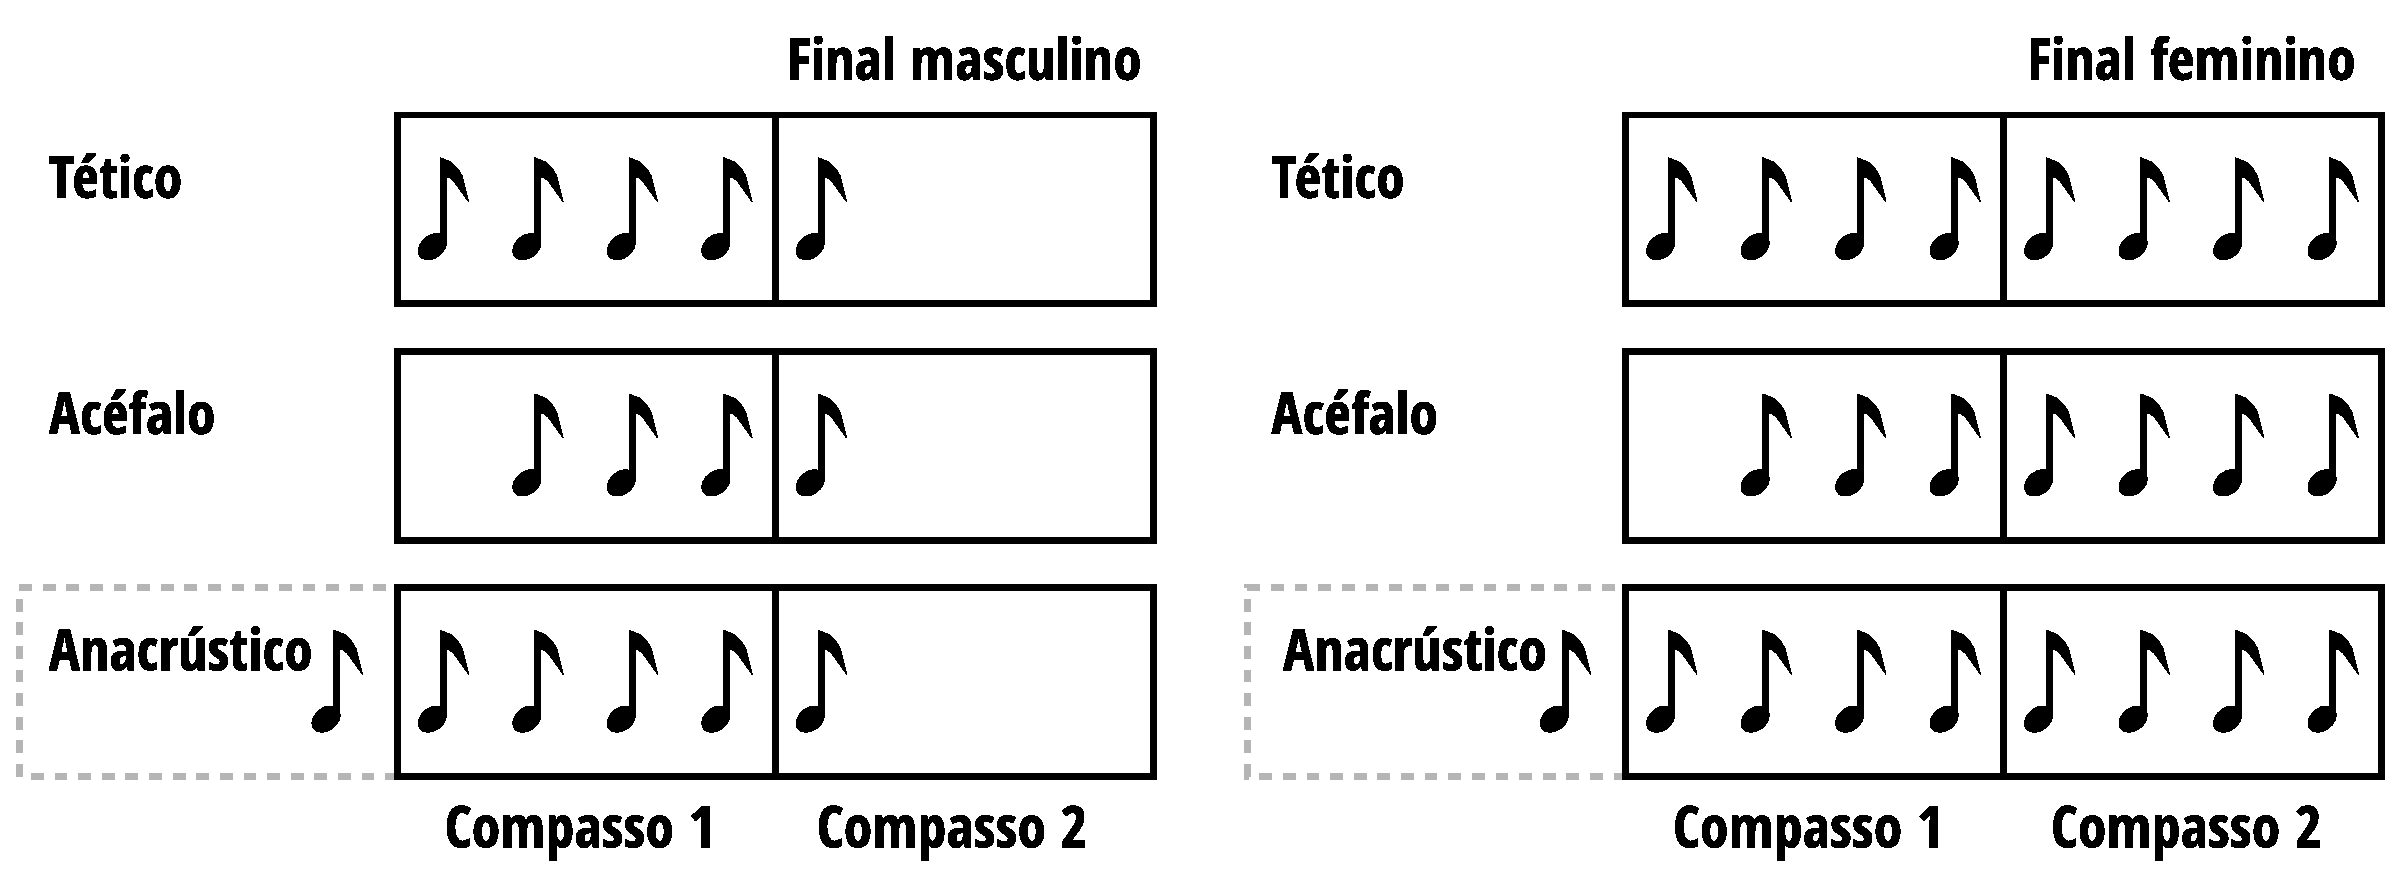
\includegraphics[width=\textwidth]{chapters/cap-musicalidade/contagemcompassosfrase.eps}
    \caption{Frases musicais com 2 compassos de comprimento.}
    \label{fig:contagemtemposfrase}
\end{figure}
É importante ressaltar que não importa a porção do compasso usado no final da frase,
pois este sempre é contado no comprimento;
mas isto não é assim no caso das notas no inicio,
pois o compasso que contem as anacruses não é computado.


\PRLsep{Detetando o inicio e o final de frase musical}


De forma geral, em músicas com textura \hyperref[subsec:monofonica]{\textbf{monofônica}} 
e \hyperref[subsec:homofonica]{\textbf{homofônica}} o acompanhamento percussivo ou harmônico 
se amolda à (única) linha melódica, 
pelo que identificar e seguir  as frases musicais pode ser mais simples no acompanhamento 
por ter uma caraterística regular e repetitiva.


%%%%%%%%%%%%%%%%%%%%%%%%%%%%%%%
\label{pos:detetandoiniciofrase}
Entre as dicas que podemos seguir para detetar o inicio de uma frase musical, encontramos que:
\begin{itemize}
\item Em musicas com uma única linha melódica, podemos detetar o inicio da frase musical,
analisando a letra ou sua melodia correspondente;
se apos uma pausa, escutamos primeiro uma nota em tempo forte (\hyperref[subsub:Tetico]{\textbf{tética}}),
então temos achado o inicio da frase e começamos a contagem desde esse compasso;
por outro lado se escutamos primeiro uma nota em tempo fraco,
devemos analisar se o inicio é \hyperref[subsub:anacrustica]{\textbf{anacrústico}} ou 
\hyperref[subsub:Acefalo]{\textbf{acéfalo}}; 
se o inicio é anacrústico, 
as notas antes do primeiro tempo forte e seu compasso são descartadas da contagem;
no caso contrario, estamos frente a um inicio acéfalo e o compasso sim é incluído na contagem. 
\item Existe geralmente, no primeiro tempo do primeiro compasso da frase, 
uma convergência de instrumentos de percussão, ou em geral do acompanhamento da melodia principal,
que provoca que este tempo forte seja percebido com maior \hyperref[sec:pos:Intensidade]{\textbf{intensidade}} 
que os outros tempos fortes da frase,
pelo que este tempo marca o inicio da contagem.
\item Na música \hyperref[subsec:homofonica]{\textbf{homofônica}} as harmonias de acompanhamento estão geralmente submetidas
à frase da melodia; assim, pela regularidade deste acompanhamento harmônico,
pode ser mais simples procurar o inicio da frase na harmonia.
\end{itemize}

%%%%%%%%%%%%%%%%%%%%%%%%%%%%%%%
\label{pos:detetandofinalfrase}
Entre as dicas que podemos seguir para detetar o final de uma frase musical, encontramos que:
\begin{itemize}
\item Geralmente entre o final de uma frase e o inicio de outra  
existe um tempo de espera maior que o visto nas notas regulares da frase.

\item Podemos detetar o final da frase se aprendemos a reconhecer os tipos de \hyperref[sec:Cadencia]{\textbf{Cadência}} 
vistas na Seção \ref{sec:Cadencia}.
\item Podemos prestar atenção ao \hyperref[ref:PontoCulminanteSuperior]{\textbf{ponto culminante superior}},
na frase musical dado que este indica que o final está próximo (ver Pag. \pageref{ref:PontoCulminanteSuperior}).
\item Podemos detetar o final da frase musical porque percebemos o enfases no inicio da seguinte frase.
\end{itemize}


\begin{example}[Músicas com frases de 4 compassos de comprimento:] ~
\label{ex:frasesde4compassos}
\begin{itemize}
\item ``Piston de gafieira'' de Billy Blanco.
\item ``Suingue de samba'' interpretado por Rogê.
\item ``Disritmia'' interpretado por Martinho da Vila.
\item ``Historia do samba'' interpretado por Joyce. % contando corporalmente é fácil de perceber.
\item ``impaciência'' interpretado por Luciana Mello.
%%%% quase regulares
\item ``Enfeitiçado'' interpretado por Aline Cardoso. 
Só tem uma frase de 3 compassos aproximadamente no meio da música.
\end{itemize}
\end{example}

\begin{comment}
\begin{tcbattention}
Podemos detetar intuitivamente o final de uma frase musical se 
interpretamos ela como se fosse uma frase falada (balbucio de uma criança) e 
percebemos nela o final de uma ideia, mais ideias na Seção \ref{subsec:fraseintuitivamente}.
\end{tcbattention}
\end{comment}

\begin{example}[Músicas com frases de 8 compassos de comprimento:] ~
\begin{itemize}
\item ``Altar particular'' interpretado por Maria Gadú. 
\item ``A cada dia que passa'' interpretado por Emílio Santiago.
\end{itemize}
\end{example}



\subsection{Separando frases intuitivamente}
\label{subsec:fraseintuitivamente}
Quando a música inclui letra é mais fácil distinguir intuitivamente  
onde inicia e finaliza uma frase,
pois nosso cérebro está treinado para perceber e processar a fala e sua estrutura;
reconhecendo automaticamente onde existem signos de pontuação como:
a virgula, o ponto e virgula, o ponto, o signo de admiração ou interrogação;
os quais descrevem finais de frases e nos indicam o tipo ou o proposito da frase e as que vem depois.

Este processamento automático não é exclusivo da fala num idioma em particular,
pois lembremos que quando escutamos a uma criança muito pequena tentando falar,
não conseguimos entender o significado dos seus balbucios, 
mas sim conseguimos separar as frases e identificar frases exclamativas e interrogativas,
frases afirmativas e suspensivas;
tudo isto sem precisar do conteúdo das palavras.

Assim, com um pouco de esforço e imaginação,
podemos supor que os sons de um instrumento musical 
são como balbucios de criança e podemos tentar extrair intuitivamente as frases musicais. 


\begin{example}[O discurso de ``la'']
\label{ex:discrusodela}
Usando unicamente a silaba ``la'', crie um discurso; por exemplo:
\begin{citando}%%
Lálala la lalá lá!\\
la lalá la lálala ...\\
la lalalá lála?\\
la lalá la lalalá.\\
\end{citando}%%
Logo proceda a ler acentuando, pausando e
executando signos de interrogação e admiração.

Perceba que o conteúdo das palavras não existe, 
porém pela expressividade na leitura é possível deduzir dos sonidos produzidos,
onde existem acentos, pausas, e signos de admiração ou interrogação.
\end{example}

\begin{example}
Na música ``Brasileirinho''  de Valdir Azevedo, 
ao tentar extrair as frases musicais, 
acontecerá o mesmo que com o discurso de ``la'' visto no Exemplo \ref{ex:discrusodela};
observaremos que:
\begin{itemize}
\item Teremos uma noção dos acentos na melodia e poderemos intuir, 
fazendo um levantamento estatístico,
em que tempo estará localizado o tempo forte. O analises será probabilístico,
pois na música existe a acentuação de tempos fracos (\hyperref[sec:contratempo]{\textbf{contratempos}}), 
pelo que se alguns tempos não cumprem com nossa predição podemos catalogar eles como contratempos.
\item Podemos perceber as pausas na melodia e deduzir que existe um final de \hyperref[sec:Frase]{\textbf{frase}} musical ou intuir o uso de uma \hyperref[fig:Cesura]{\textbf{cesura}}.
\item Também podemos perceber diferentes formas de finalizar uma frase, 
que na linguagem falada associaríamos com o uso ou não de signos de admiração e exclamação;
no âmbito da música, temos algo similar mediante o uso das \hyperref[sec:Cadencia]{\textbf{cadências}}.
Assim, cada tipo de cadência nos dará uma ideia diferente da função que cumpre a frase no discurso da peça musical 
e se existirá ou não uma frase de resposta.
\end{itemize}
\end{example}
